\documentclass[a4j, fleqn, 12pt]{jsreport}
\usepackage{bm}
\usepackage[dvipdfmx]{graphicx}
\usepackage{listings}
\usepackage{fancyhdr}
\usepackage{amsmath}
\usepackage{bm}
\usepackage{setspace}
\usepackage{url}
\usepackage{multirow}
\usepackage{multicol}
\usepackage{float}
\usepackage{pifont}

\usepackage{STY/h25-GT}
\usepackage{STY/arydshln}

\usepackage{enumerate}
\def\circledenumerate#1{\textcircled{\scriptsize #1}}
\def\MARU#1{\leavevmode \setbox0\hbox{$\bigcirc$}
\copy0\kern-\wd0 \hbox to\wd0{\hfil{#1}\hfil}}

\usepackage{caption}
\captionsetup{font=small, labelfont=small}

\lstset{
    basicstyle={\ttfamily},
    identifierstyle={\small},
    commentstyle={\smallitshape},
    keywordstyle={\small\bfseries},
    ndkeywordstyle={\small},
    stringstyle={\small\ttfamily},
    frame={tb},
    breaklines=true,
    columns=[l]{fullflexible},
    numbers=left,
    xrightmargin=0zw,
    xleftmargin=3zw,
    numberstyle={\scriptsize},
    stepnumber=1,
    numbersep=1zw,
    lineskip=-0.5ex,
    keepspaces=true,
    language=c
}
\renewcommand{\lstlistingname}{リスト}
\makeatletter
\newcommand{\figcaption}[1]{\def\@captype{figure}\caption{#1}}
\newcommand{\tblcaption}[1]{\def\@captype{table}\caption{#1}}
\makeatother

\renewcommand{\chaptermark}[1]{\markboth{#1}{}}
\renewcommand{\sectionmark}[1]{\markright{#1}{}}

\reportname{令和3年度電子制御工学科卒業論文}
\reporttitle{情報端末の内蔵カメラを用いた運動再現システム}
\reportdate{2022/02/21}
\autheraff{
長岡工業高等専門学校\\
電子制御工学科\\
制御工学研究室\\
(指導教員    外山 茂浩)
}
\reportauther{平田 蓮}

\pagestyle{fancy}
\rhead{\thesection\, \rightmark}
\lhead{第\ \thechapter\ 章\, \leftmark}
\rfoot{制御工学研究室}

\begin{document}
\pagenumbering{roman}
\maketitle
\tableofcontents
\cleardoublepage
\pagenumbering{arabic}

\chapter{序論} \label{cha:background}
    \section{スポーツ指導の現状} \label{sec:current}
        現在、スポーツ指導の現場では、従来から行われてきた、
        熟練した指導者の「目」に基づく「感覚的な指導」に比べ、
        カメラのような機械の「目」を用いてデータ化した選手の動きなどに基づく
        「定量的な指導」に注目が集まっている\cite{JSA}。

        選手の動きをデータ化するにあたって、様々なアプローチが行われてきた\cite{Watanabe}。
        この「データ」には、球技におけるボールの位置、選手の位置、
        選手の姿勢などが含まれるが、
        本研究ではバレーボールの試合中における、特に選手の位置に注目を絞る。

    \section{Data Volley} \label{sec:Data Volley}
        バレーボールの解析に用いるツールとして、Data Volley
        \footnote{https://www.dataproject.com/Products/EN/en/Volleyball/DataVolley4}を紹介する。
        これはイタリアのGenius Sports Italy社が開発するソフトウェアで、
        現在バレーボール業界で広く用いられている。

        図\ref{fig:Data Volley}にData VolleyのGUIを示す。
        これはアナリストと呼ばれる専門家やコーチが用いるソフトウェアで、
        各選手のポジションをあらかじめ登録し、
        コマンドで選手がボールに触れたときの行動を試合を観ながらリアルタイムで入力する。
        それに基づいて、プレイの決定率や、
        選手たちの位置をあとから見直せるものである。

        \begin{figure}[ht]
            \centering
            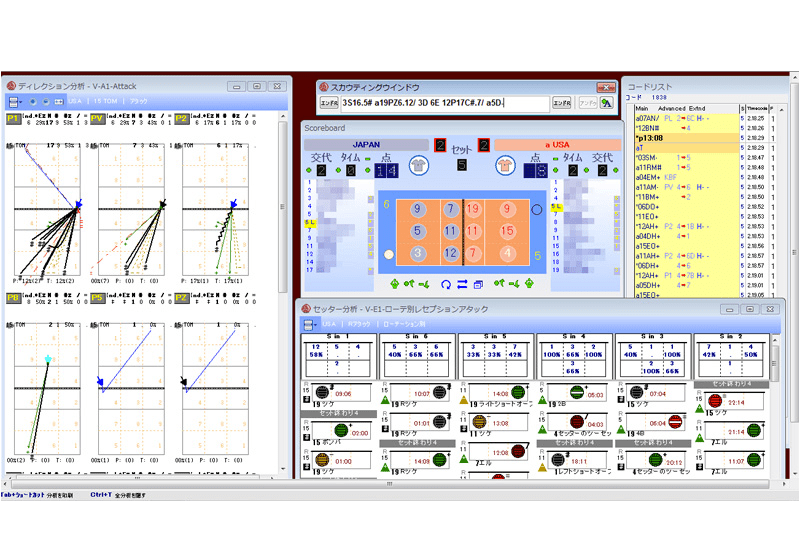
\includegraphics[width=0.8\hsize]{images/data-volley.png}
            \caption{Data VolleyのGUI}
            \label{fig:Data Volley}
        \end{figure}
        
        しかし、Data Volleyには次に示すような欠点が挙げられる。

        \begin{itemize}
            \item 複雑な入力コマンド
            \item 瞬間的なプレイの判断の要求
            \item 記録される位置の精度の低さ
            \item 人的入力ミス
        \end{itemize}

        1つ目は「複雑な入力コマンド」である。
        以下に、入力コマンド例を2つ示す。

        \begin{verbatim}
15S.14#K1a26P4.17+14Q15#.K3a25E.
3S16.5#a19PZ6.12/3D6E12P17C#.7a5D.
        \end{verbatim}

        これらの意味は割愛するが、
        それぞれ1ラリー中での両チームのボールのやりとりを示している。
        このような複雑なコマンドを覚えるだけでなく、
        選手たちのプレイを見ながら入力を行う必要があるため、
        ある程度の練習が必要である。

        2つ目は「瞬間的なプレイの判断の要求」である。
        Data Volleyはバレーボールの試合中のプレイを解析するため、
        入力を行うユーザにはもちろんバレーボールの知識が要求される。
        さらに、入力にはプレイの種類だけでなく、
        ユーザからみたその評価も含むため、
        バレーボールのルールを知っているだけでなく、
        プレイの評価もできることがユーザに求められる。
        これは、先述の「複雑な入力コマンド」に重ね、Data Volleyの使用の敷居を高めており、
        \ref{sec:current}節にて述べたように、
        このソフトウェアのユーザをアナリストやコーチに限定しまっている要因である。

        3つ目は「記録される位置の精度の低さ」である。
        Data Volleyでは、図\ref{fig:area}に示すように、
        コートの片面を$6\times 6$に36等分して扱う。
        バレーボールコートの片面は9m四方であるため、
        Data Volleyで記録される位置の最小単位は1.5m四方ということになる。

        \begin{figure}[ht]
            \centering
            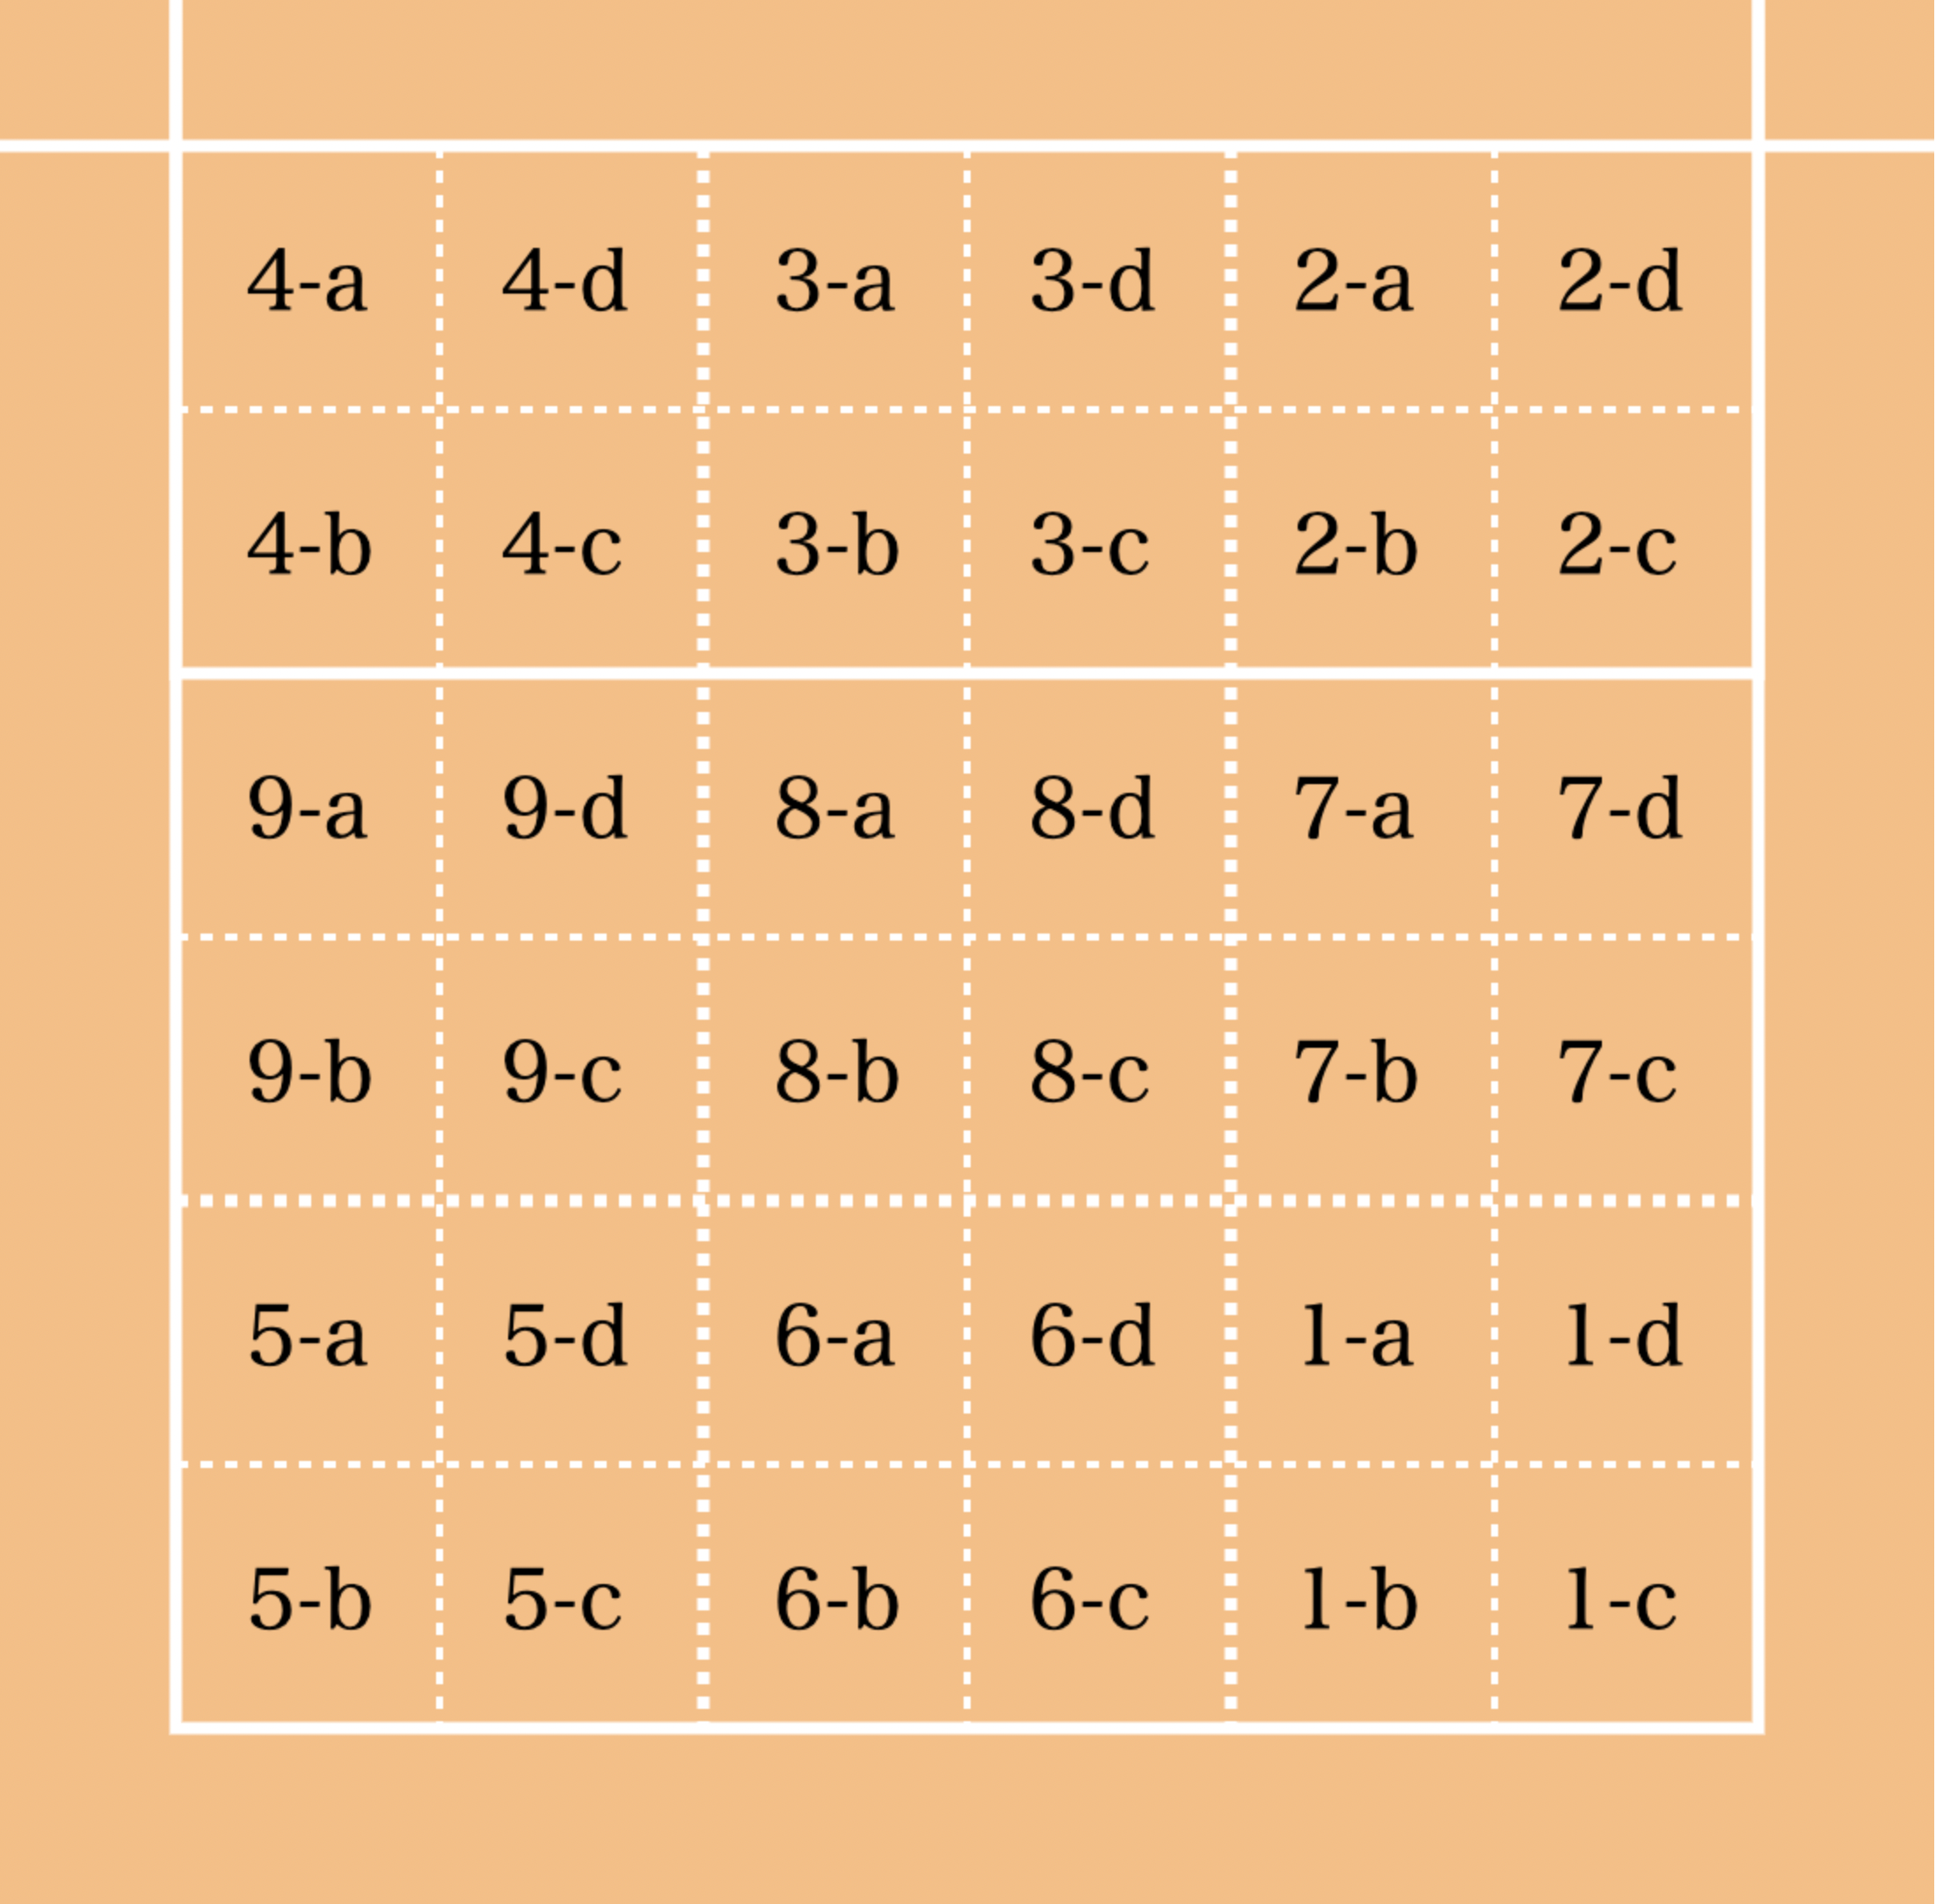
\includegraphics[width=0.8\hsize]{images/areas.png}
            \caption{Data Volleyにおけるコートの分割}
            \label{fig:area}
        \end{figure}

        また、ボールに触れていない選手の位置は入力しないため、
        ボールに触れた瞬間でしか選手の位置を見直せないことも同様に欠点である。

        最後に「人的入力ミス」を挙げた。これはいうまでもなく、
        ユーザがコマンドを入力をする際に起こすミスのことである。
        例えば背番号の\verb|4|と\verb|5|や、
        レシーブの一種を表す\verb|D|と返球の一種を表す\verb|F|は
        最も一般的なQWERTY配列のキーボード上では隣り合っているが、
        これらが間違って入力された場合は
        大きく意味が異なり致命的である。

    \section{データを用いたバレーボール指導}
        本節では、本研究で注目する、「選手の位置」に基づき行われる指導の例を示す。

        \begin{itemize}
            \item 相手の攻撃に対する防衛陣形の指導
            \item 相手の陣形に対する攻撃の指導
            \item コート内での選手のエリア管理
        \end{itemize}

        これらはどれもチーム全員の位置情報に基づくため、
        Data Volleyでは実現ができない指導である。

        現状、多くのチームは動画を後から見直し、ホワイトボードなどを用いてこれを行っている。

    \section{本研究が目指すシステム} \label{sec:system}
        本研究の目的を、\ref{sec:current}節でも述べたように、
        選手の位置に注目した解析システムの構築とする。
        具体的には、バレーボール選手の位置を推定するシステムを目指す。
        ここでいう「位置」とは、
        選手の現実世界における床上の位置である。
        解析対象には、現在Data Volleyのユーザが最も用いている
        情報端末を用いて撮影したバレーボールの試合映像を用いる。
        本研究では、Apple社のiPad Proを用いて撮影したFHDの映像を用いた。
        さらに、Data Volleyのようなシステムの構築の基礎とするため、
        \ref{sec:Data Volley}節に示したData Volleyの欠点を踏まえて、
        「(できる限り)人の手を介さない」、さらに、「扱いやすい」システムを目指す。
        ここでいう「扱いやすさ」とは、活用ができるユーザ数が限られてしまっている
        Data Volleyに比べて、より一般的に多くの人が使えることを指す。

        \subsection {先行研究との比較}
            中井ら\cite{Nakai}は、2台のカメラを用いてバレーボールコート内の
            選手の動きを解析するためのキャリブレーション手法を提案した。
            この手法を用いると、コート内の選手及びボールの位置を3次元でデータ化できる。
            本研究では先述したように選手の床上の位置を推定するため、
            ボールの位置を推定しない点と、推定位置が2次元である点で劣る。

            しかし、カメラを複数台使って撮影を行う場合、
            それぞれのカメラの映像の時間同期や、
            キャリブレーションが必要であり一般的なスポーツクラブなどで使用するには不便である。
            本研究ではカメラを1台のみ使う点と、
            カメラの位置が自由である点に優位性を見出した。
            
            北原ら\cite{Kitahara}は、他視点カメラを用いて、
            スポーツを自由視点から見直す手法を提示した。
            この研究は、選手の動きを具体的にデータ化しないが、
            選手の動きを見直し、
            指導に役立てるという動機に別方向からのアプローチを行っている。

    \section{本論文の構成}
        最後に、本論文の構成を示して序論を締めくくる。
        第\ref{cha:background}章では、本研究の背景及び目的を述べた。
        第\ref{cha:detect}, \ref{cha:pose}, \ref{cha:result}章では、
        この目的を実現するためのアルゴリズムを述べる。
        第\ref{cha:result}章ではさらに、
        これらのアルゴリズムを用いて得られた結果を述べている。
        第\ref{cha:evaluation}章では、
        得られた結果の精度評価を行っている。
        最後に、第\ref{cha:epilogue}章では
        本研究のまとめと課題、及び展望を述べている。

        また、付録\ref{app:3D}, \ref{app:code}ではそれぞれ、
        \ref{sec:prospect}節で述べる選手の3次元姿勢の推定と、
        本研究で作成したプログラムのソースコードを紹介している。

\chapter{映像内のコートの検出} \label{cha:detect}
    映像内の選手の実際の位置を推定するためには、
    映像内でコートがどこに写っているかの情報が必要である。
    これを得る方法の例として、以下が挙げられる。

    \begin{itemize}
        \item 画像処理を用いたコートラインの検出
        \item 物体検出アルゴリズムを用いたポールやアンテナの検出
    \end{itemize}

    1つ目は「画像処理を用いたコートラインの検出」である。
    本研究では体育館で撮影された映像を用いる。
    バレーボールの競技専用ではない一般的な体育館には、
    バレーボール以外の競技に用いるラインも引かれている。
    そのため、この方法は正確性に欠けるとして使用を見送った。

    2つ目は「物体検出アルゴリズムを用いたポールやアンテナの検出」である。
    この方法は、物体検出アルゴリズムを用いて映像内に映るポールやアンテナなどの目印となる物体を
    検出することで、映像内のコートの位置を推定する。
    これについて\ref{sec:antenna}節で詳しく述べる。

    \section{アンテナを用いた検出} \label{sec:antenna}
        本研究では物体検出アルゴリズムの一つである、YOLO\cite{Joseph}を用いた。
        YOLOは、画像を入力とする物体検出アルゴリズムである。
        これを利用するため、
        本研究では映像を各フレームごとに画像に分けて処理を行う。

        また、ポールやネットなど、
        バレーボールコートの目印となる物体はアンテナの他にもあるが、
        これらはコートごとに色や形が変わるため、
        本研究では見た目が
        統一されているアンテナの検出を目指した。

        アンテナはネットに2本設置されている。
        これらを検出することで、
        その位置関係や向きからコートの位置を推定する。

        YOLOは、機械学習を用いており、
        学習済みモデルが配布されている\footnote{https://github.com/pjreddie/darknet}。
        しかし、これらを学習する際にバレーボールのアンテナの画像は
        用いられていないため、これらでアンテナを検出することは不可能である。
        そのため、本研究ではアンテナの画像を用いたデータセットを作成し、
        新たなモデルを学習した。
        これらについて\ref{subsec:dataset}, \ref{subsec:antenna_result}項で詳しく述べる。

        \subsection{データセットの作成} \label{subsec:dataset}
            本研究では、体育館で撮影した映像を解析するため、
            体育館の画像を背景とし、それにアンテナの画像を貼り付けた画像を作成した。
            図\ref{fig:pasted}に、作成した画像例を示す。
            アンテナの数、向き、大きさに差異を持たせ、10000枚の画像と、
            それぞれの画像について、そこにアンテナが写っているかを記録したファイルを作成した。

            \begin{figure}[ht]
                \centering
                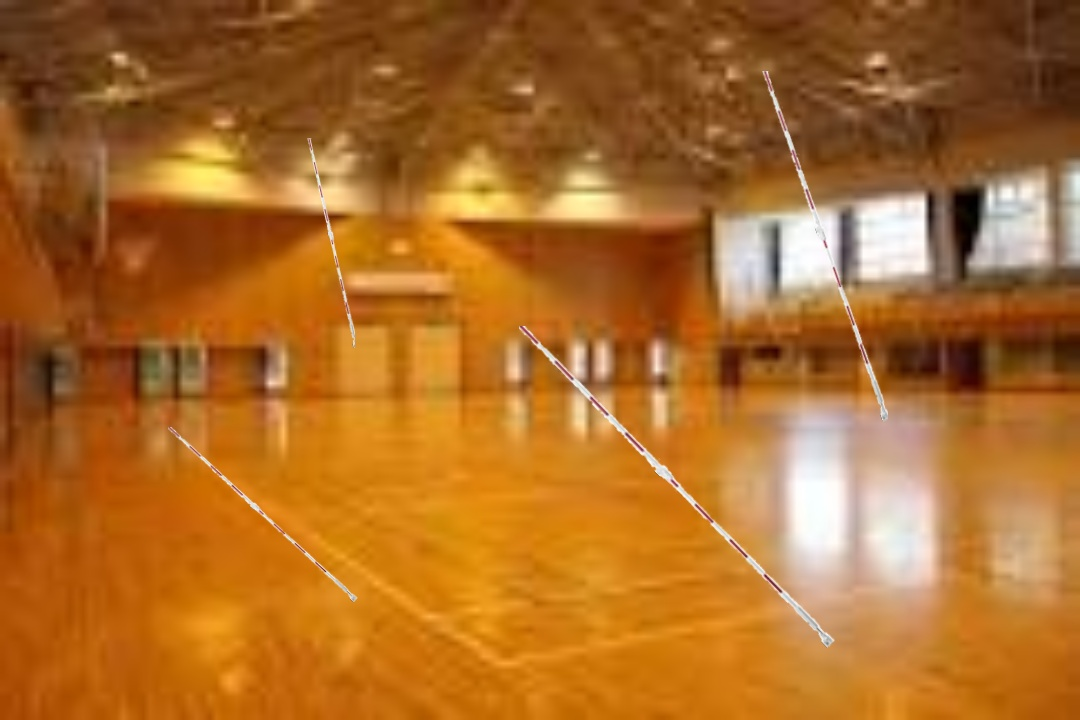
\includegraphics[width=0.8\hsize]{images/00075.jpg}
                \caption{作成した画像}
                \label{fig:pasted}
            \end{figure}

        \subsection{学習結果} \label{subsec:antenna_result}
            モデルは、YOLOで用いられるモデルのうちCOCOデータセット\cite{Microsoft}において
            最も高いスコアを残しているYOLOv5x6を用いた。
            本研究では転移学習ではなく、モデルのパラメータを乱数で初期化し、
            一から作成したデータセットを用いて学習させた。

            結果として、mAPにおいて97.5\%を達成することができた。
            しかしながら、アンテナの検出はうまくいったものの、
            2本のアンテナの位置、大きさ、角度から映像内に写るコートの位置を推定した結果、
            コートネットに対して正面、または垂直に撮影した映像からは
            上手くコートの位置を推定することができたが、
            斜めに撮影した映像では不可能であった。
            本研究ではカメラの位置の自由度に新規性を見出すため、アンテナなどの目印を用いた
            コートの自動検出を断念した。

    \section{GUIを用いた手動指定}
        \ref{subsec:antenna_result}項の結果を踏まえて、
        本研究では、映像内のコートの位置は既知であるとして
        研究を進めることにした。
        これを実現するために、使用者が手動でコートの隅を指定できるGUIを作成した。
        図\ref{fig:GUI}に作成したGUIを示す。
        画面をクリックしてコートの隅の位置を指定すると、
        青いマーカーと直線でそれが表示される。

        \begin{figure}[ht]
            \centering
            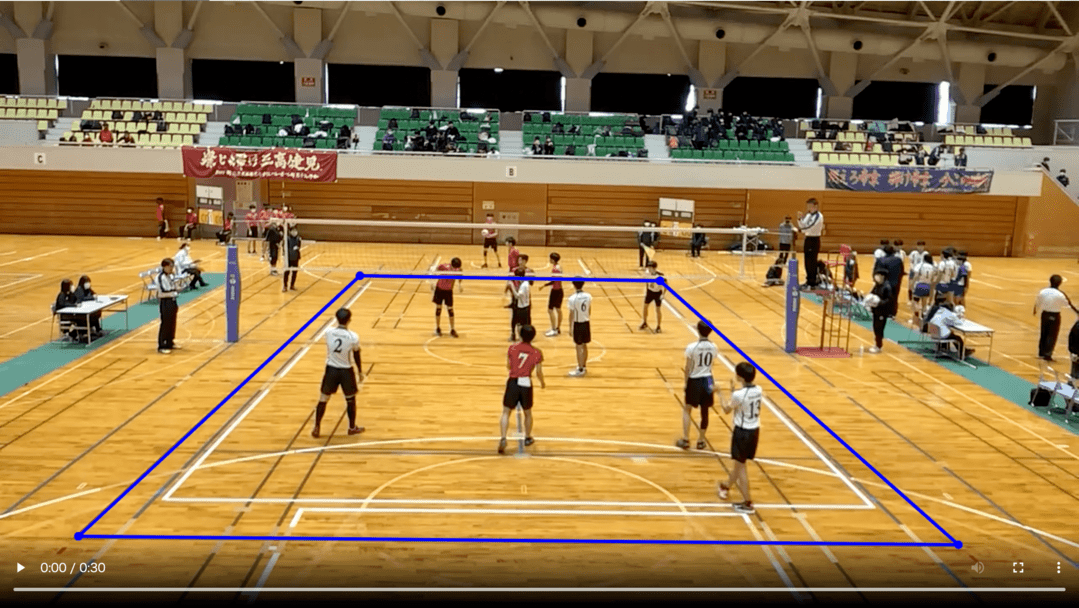
\includegraphics[width=0.8\hsize]{images/gui.png}
            \caption{作成したGUI}
            \label{fig:GUI}
        \end{figure}

\chapter{映像内の選手の検出} \label{cha:pose}
    第\ref{cha:detect}章では、映像内のコートの検出について述べた。
    次に、本章では映像内の選手の検出について述べる。
    本研究では姿勢検出アルゴリズムである
    OpenPose\cite{Zhe}とAlphaPose\cite{Hao}を用いてこれを行った。
    \ref{sec:antenna}節で触れたYOLOなどの物体検出アルゴリズムを用いても
    映像内の選手は検出可能であるが、
    選手の位置だけでなく姿勢の情報も取得するために姿勢検出アルゴリズムを用いた。
    これについては、\ref{sec:prospect}節で詳しく述べる。

    OpenPoseとAlphaPoseはどちらも画像を入力とするため、
    \ref{sec:antenna}節でYOLOを用いた際と同様に各フレームに分けて処理を行った。
    AlphaPoseは、映像内で連続する画像を入力すると、
    それらに写る選手たちの姿勢だけでなく、
    片方の画像に写る選手と、
    もう一方の画像に写る同選手の対応も出力される。
    これを用いて、選手の追跡が可能である。
    本研究では始めはOpenPoseを用いて解析を行っていたが、
    バレーボールのようなチームスポーツを解析するにあたって、
    その瞬間ごとの選手の位置だけでなく、
    選手の追跡が必要であると考え、
    AlphaPoseを用いた解析に移行した。

    \section{AlphaPoseを用いた選手の検出}
        図\ref{fig:frame}, \ref{fig:posed}に
        本研究で解析に用いた映像に含まれる画像と、
        それをAlphaPoseで解析した結果を示す。

        \begin{figure}[ht]
            \begin{minipage}{0.49\hsize}
                \centering
                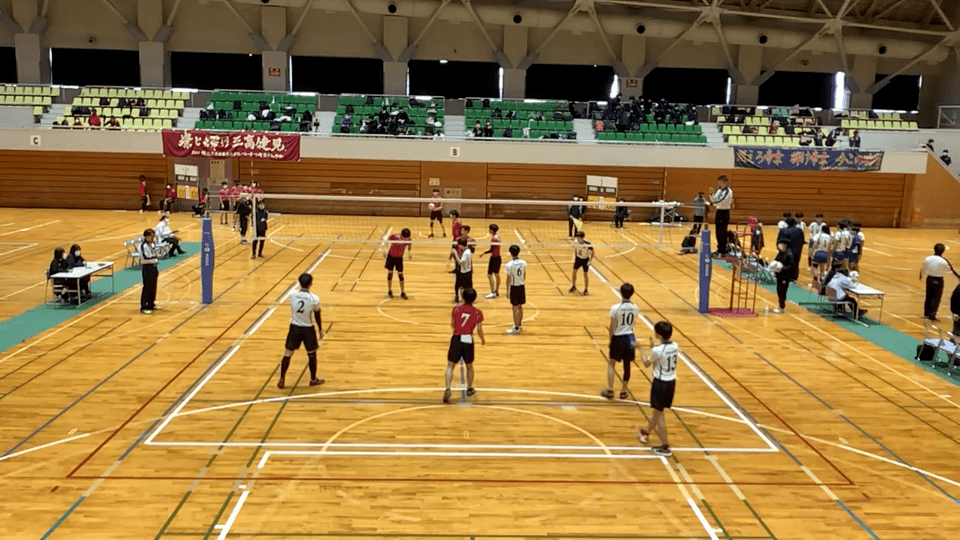
\includegraphics[width=1\hsize]{images/frame.png}
                \caption{バレーボールの試合の様子}
                \label{fig:frame}
            \end{minipage}
            \begin{minipage}{0.49\hsize}
                \centering
                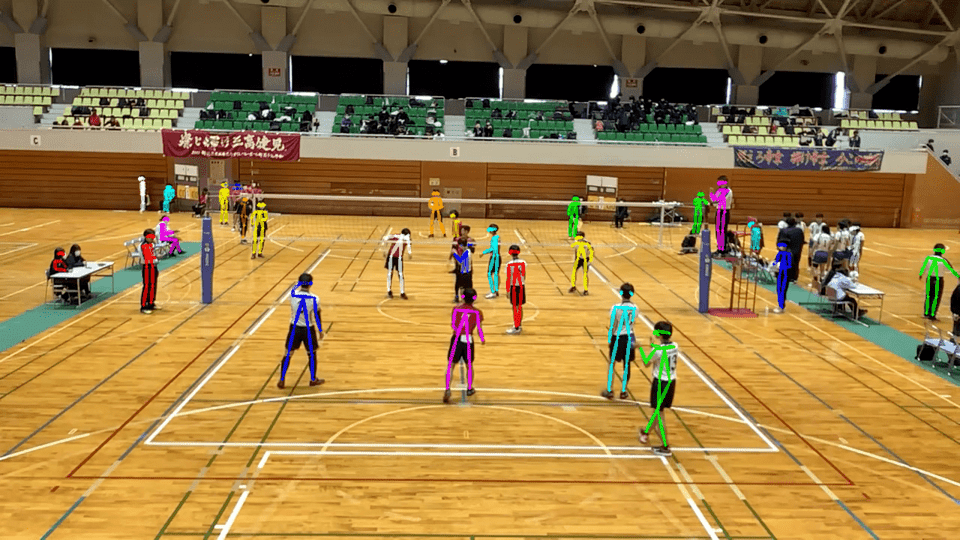
\includegraphics[width=1\hsize]{images/posed.png}
                \caption{AlphaPoseを用いた解析結果}
                \label{fig:posed}
            \end{minipage}
        \end{figure}

        図に示したように、
        画像内の選手の姿勢情報が得られる。
        AlphaPoseは姿勢情報として、
        画像内の人物それぞれについて17個の関節点の位置を出力する。
        AlphaPoseの出力は画像内の各人物に対して

        \begin{verbatim}
{
    "image_id" : 画像名,
    "category_id" : 1,
    "keypoints" : 各関節の位置,
    "score" : 人物の最もらしさ
}
        \end{verbatim}
        という形式で得られる。「各関節の位置」は、
        17個の関節点それぞれに対して画像内の横、縦方向座標、最もらしさの3要素を含んだ、
        51要素の配列である。

    \section{推定に用いる情報の抽出}
        AlphaPoseで得られた姿勢情報から、
        選手の位置を推定するのに用いる情報を抜き出す。
        本研究では、画像内における選手の床上の位置として両足の中点を用い、
        選手の両足が床についている前提で解析を行った
        (空中にいる選手については\ref{sec:problems}節で詳しく述べる)。
        図\ref{fig:marker}に、図\ref{fig:frame}に写る選手について、
        AlphaPoseを用いて得られた左右足首の座標の中点に緑色のマーカーで
        印をつけたものを示す。

        \begin{figure}[ht]
            \centering
            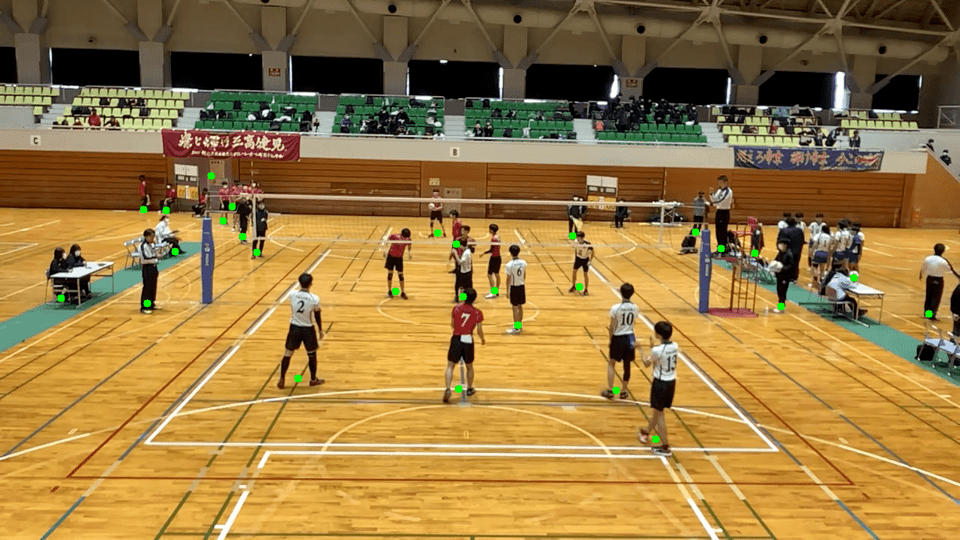
\includegraphics[width=0.8\hsize]{images/pointed.png}
            \caption{選手の床上の位置}
            \label{fig:marker}
        \end{figure}

\chapter{射影変換を用いた選手の位置推定} \label{cha:result}
    第\ref{cha:detect}, \ref{cha:pose}章では、
    映像内のコートと選手の位置を検出した。
    本章では、
    これらを用いて射影変換を行い、選手の実際の位置を推定する。

    \section{射影変換}
        射影変換は、四角形を別の四角形へと変換するアルゴリズム\cite{kashika}である。
        4点$(x_{11}, y_{11})$, $(x_{12}, y_{12})$,
        $(x_{13}, y_{13})$, $(x_{14}, y_{14})$
        からなる四角形から、
        別の4点$(x_{21}, y_{21})$, $(x_{22}, y_{22})$, $(x_{23}, y_{23})$,
        $(x_{24}, y_{24})$からなる四角形への変換を考える。

        変換前の四角形の頂点$(x_1, y_1)$から、
        それに対応する変換後の頂点$(x_2, y_2)$への変換は、
        変換行列$A$を用いて次のように表せる。
        \begin{eqnarray*}
            \left(
                \begin{array}{c}
                    x^\prime \\
                    y^\prime \\
                    s
                \end{array} 
            \right) &=& A \left(
                \begin{array}{c}
                    x_1 \\
                    y_1 \\
                    1
                \end{array}
            \right) \\
            \left(
                \begin{array}{c}
                    x_2 \\
                    y_2
                \end{array} 
            \right) &=& \frac{1}{s} \left(
                \begin{array}{c}
                    x^\prime \\
                    y^\prime
                \end{array} 
            \right)
        \end{eqnarray*}

        この式を4つ全ての頂点について立て、
        解くと、$A$の成分が計算できる。

        選手の実際の位置を推定するにあたり、
        変換前の四角形を第\ref{cha:detect}章で述べた
        映像内のコートとし、変換後の四角形を上から見た実際のコートの形として
        変換を行った。
        バレーボールコートは9m$\times$18mの長方形であるため、
        後者の四角形の頂点を$\{(0, 0), (0, 18), (9, 18), (9, 0)\}$に設定した。
        計算した変換行列を用いて、図\ref{fig:marker}に射影変換を施したものを
        図\ref{fig:transformed}に示す。

        \begin{figure}[ht]
            \centering
            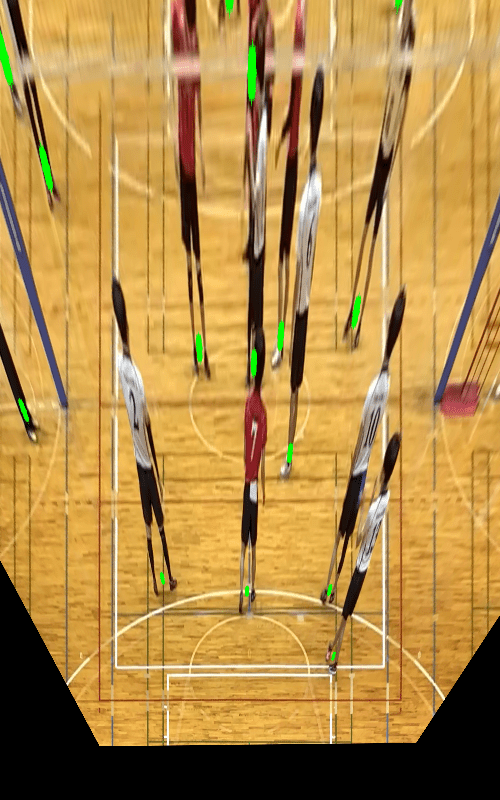
\includegraphics[width=0.5\hsize]{images/warped.png}
            \caption{射影変換を施した試合の様子}
            \label{fig:transformed}
        \end{figure}

        射影変換を行った際に、四角形の変形と同時に、
        マーカーも移動している。
        本研究では、このように、
        画像内の選手の位置を射影変換した点を選手の実際の位置として推定を行った。

    \section{推定結果}
        図\ref{fig:estimated}に図\ref{fig:frame}に写る選手の実際の位置を推定した結果を示す。

        \begin{figure}[ht]
            \centering
            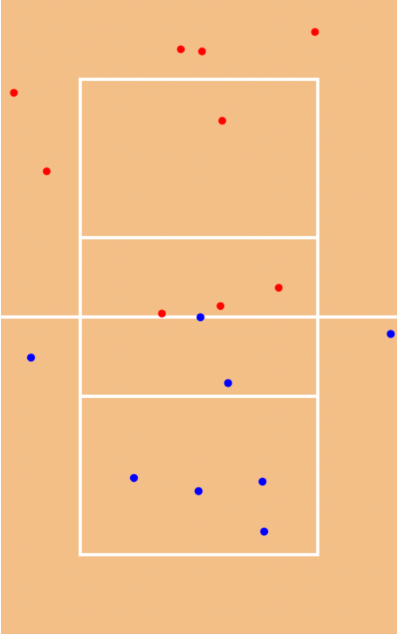
\includegraphics[width=0.5\hsize]{images/estimated.png}
            \caption{選手の位置の推定結果}
            \label{fig:estimated}
        \end{figure}

        \subsection{実行時間}
            本研究では、遠隔授業期間中も研究に専念するために、
            AlphaPoseの実行環境を、
            Google社が提供するクラウドサービスである
            Google Colaboratory
            \footnote{https://colab.research.google.com}
            を用いて構築した。
            本環境では、AlphaPoseによる解析と、
            射影変換を用いた選手の位置推定を合わせて、
            1フレーム当たり約0.010秒で処理を行うことができた。
            この環境では毎秒約100フレームを処理できることになるが、
            一般的な映像は毎秒30フレームであるため、
            リアルタイム処理に留まらず、
            録画映像に対する倍速解析が可能であると予想する。

\chapter{推定した選手の位置の精度評価} \label{cha:evaluation}
    推定した選手の位置と、
    そのときに選手が実際にいた位置を比較して本研究で提示したアルゴリズムによる推定精度を評価した。

    \section{精度評価に用いる基準点}
        評価を行うにあたって、実際の選手の位置が必要であるが、
        選手の位置を正確に追跡することは困難であるため、
        コート内に基準点を設定し、
        そこに選手がいた瞬間に注目した。
        図\ref{fig:points}, \ref{fig:on_point}に、
        設定した基準点と、ある選手が基準点1にいる瞬間の様子を示す。

        \begin{figure}[ht]
            \begin{minipage}{0.49\hsize}
                \centering
                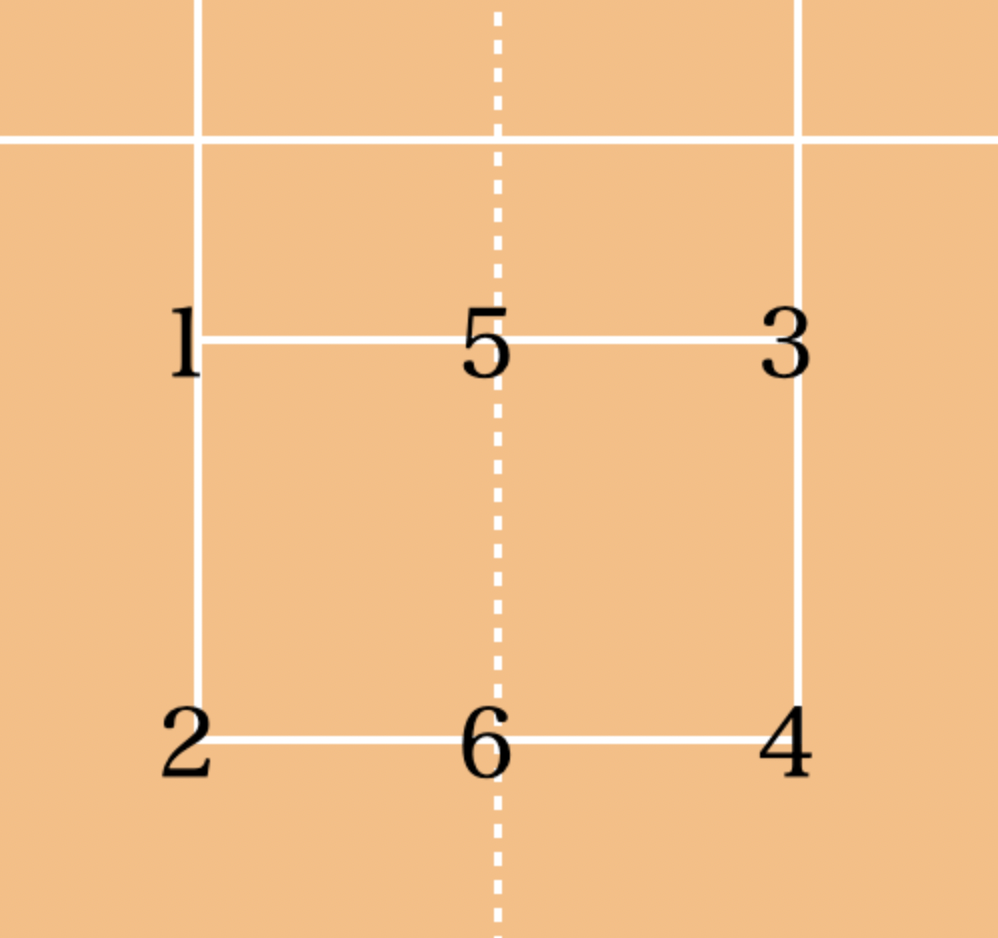
\includegraphics[width=1\hsize]{images/points.png}
                \caption{精度評価のために設定した基準点}
                \label{fig:points}
            \end{minipage}
            \begin{minipage}{0.49\hsize}
                \centering
                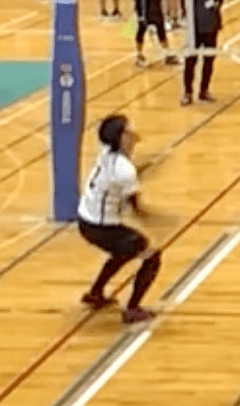
\includegraphics[width=0.7\hsize]{images/appeared.png}
                \caption{基準点1にいる選手}
                \label{fig:on_point}
            \end{minipage}
        \end{figure}

    \section{精度の評価結果}
        図\ref{fig:on_point}のように、
        映像内の選手が基準点にいる瞬間について実際の選手の位置と
        推定した位置の距離を誤差とし、基準点ごとに平均値を算出した。
        コートに対するカメラの位置による精度の変化を見る、
        図\ref{fig:camera}に示すように3箇所から撮影した映像を評価に用いた。
        その際、カメラとコートの中心の距離は20mに統一した。
        表\ref{tab:accuracy}に、評価結果を示す。
        誤差平均値の他に、括弧内に計算に用いたデータのサンプル数を示してある。
        表より、誤差は高々35cm程度に収まっていることがわかる。

        \begin{figure}[ht]
            \centering
            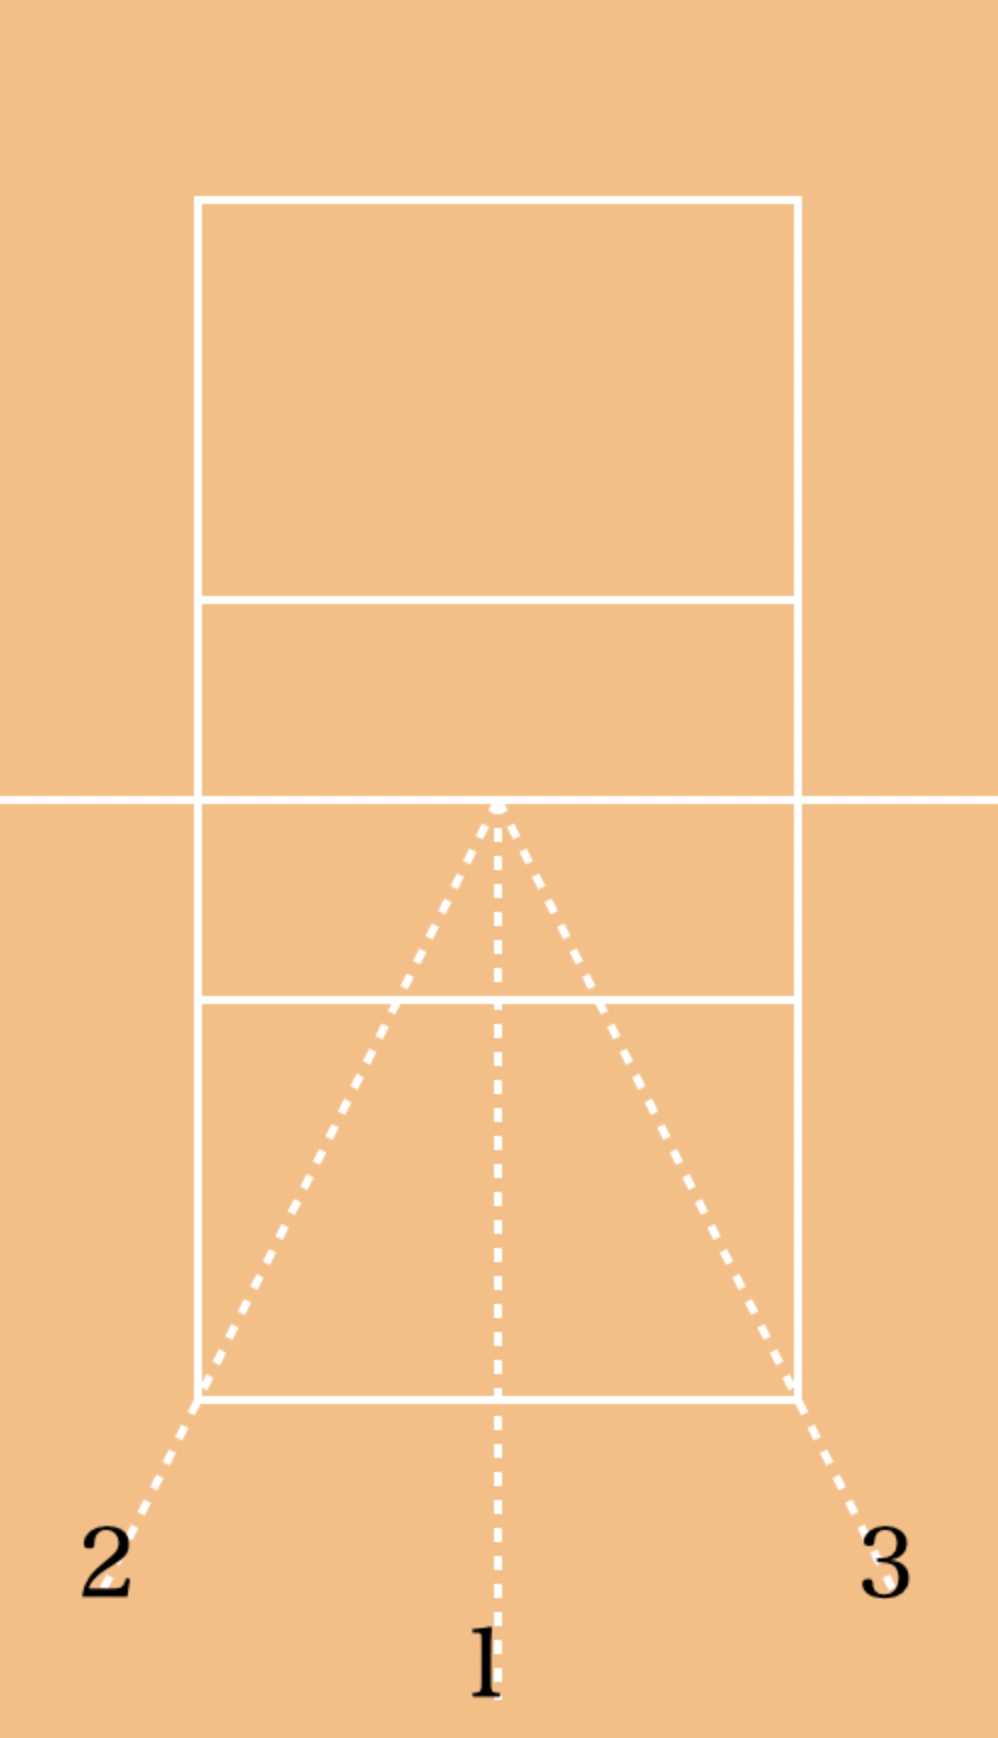
\includegraphics[width=0.5\hsize]{images/camera.png}
            \caption{精度評価に用いた映像の撮影位置}
            \label{fig:camera}
        \end{figure}

        \begin{table}[ht]
            \centering
            \caption{各基準点についての誤差の平均値[cm]}
            \label{tab:accuracy}
            \small
            \begin{tabular}{c|c||llllll} \hline
                撮影位置 & コート & \multicolumn{1}{c}{1} & \multicolumn{1}{c}{2} & \multicolumn{1}{c}{3} & \multicolumn{1}{c}{4} & \multicolumn{1}{c}{5} & \multicolumn{1}{c}{6} \\ \hline\hline
                \multirow{2}{*}{1} & 手前 & 15 \footnotesize{(127)} & 18 \footnotesize{(74)} & 14 \footnotesize{(109)} & 12 \footnotesize{(56)} & 13 \footnotesize{(387)} & 10 \footnotesize{(133)} \\
                & 奥 & 27 \footnotesize{(103)} & 32 \footnotesize{(55)} & 24 \footnotesize{(112)} & 29 \footnotesize{(78)} & 19 \footnotesize{(256)} & 28 \footnotesize{(105)} \\ \hline
                \multirow{2}{*}{2} & 手前 & 13 \footnotesize{(34)} & 12 \footnotesize{(21)} & 16 \footnotesize{(25)} & 14 \footnotesize{(15)} & 15 \footnotesize{(106)} & 13 \footnotesize{(43)} \\
                & 奥 & 18 \footnotesize{(36)} & 20 \footnotesize{(23)} & 25 \footnotesize{(18)} & 32 \footnotesize{(19)} & 23 \footnotesize{(89)} & 28 \footnotesize{(38)} \\ \hline
                \multirow{2}{*}{3} & 手前 & 17 \footnotesize{(23)} & 15 \footnotesize{(19)} & 13 \footnotesize{(37)} & 13 \footnotesize{(20)} & 14 \footnotesize{(98)} & 14 \footnotesize{(46)} \\
                & 奥 & 25 \footnotesize{(18)} & 30 \footnotesize{(22)} & 16 \footnotesize{(33)} & 22 \footnotesize{(25)} & 22 \footnotesize{(85)} & 27 \footnotesize{(38)} \\ \hline
            \end{tabular}
        \end{table}

        \ref{subsec:distance}, \ref{subsec:distribution}項で、
        基準点とカメラの距離と誤差の関係、及び、各基準点ごとの推定位置の分布について述べる。
        また、先述のカメラの位置による精度の変化は確認できなかった。

        \subsection{基準点とカメラの距離と誤差の関係} \label{subsec:distance}
            図\ref{fig:graph}に、
            表\ref{tab:accuracy}から作成した、
            カメラと基準点の距離とその基準点での誤差の関係を示す。

            \begin{figure}[ht]
                \centering
                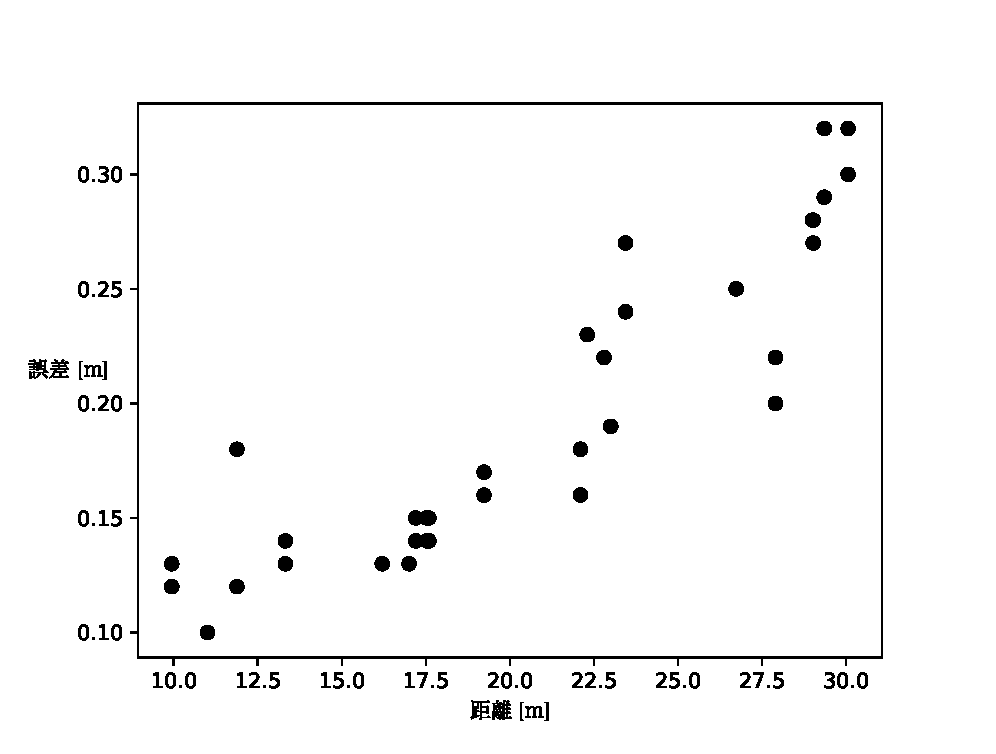
\includegraphics[width=0.8\hsize]{images/scat.eps}
                \caption{距離と誤差の関係}
                \label{fig:graph}
            \end{figure}

            図より、カメラと基準点の距離が増加するほど
            その基準点での誤差も増加している傾向が見られる。
            AlphaPoseによる選手の位置の誤差は画像のどの位置でも同等に現れる。
            映像内ではカメラから遠いものほど小さく写るため、
            射影変換を行うと相対的に遠い地点で大きな誤差が表れ、
            この結果になったと考えられる。

        \subsection{推定位置の分布} \label{subsec:distribution}
            図\ref{fig:distribution1}, \ref{fig:distribution2}, \ref{fig:distribution3}に、
            1の位置から撮影した映像における、手前コートの基準点1、
            奥コートの基準点2, 3での推定位置の分布を示す。
            赤い点が基準点の位置で、青い点が推定位置である。

            \begin{figure}[ht]
                \begin{minipage}{0.32\hsize}
                    \centering
                    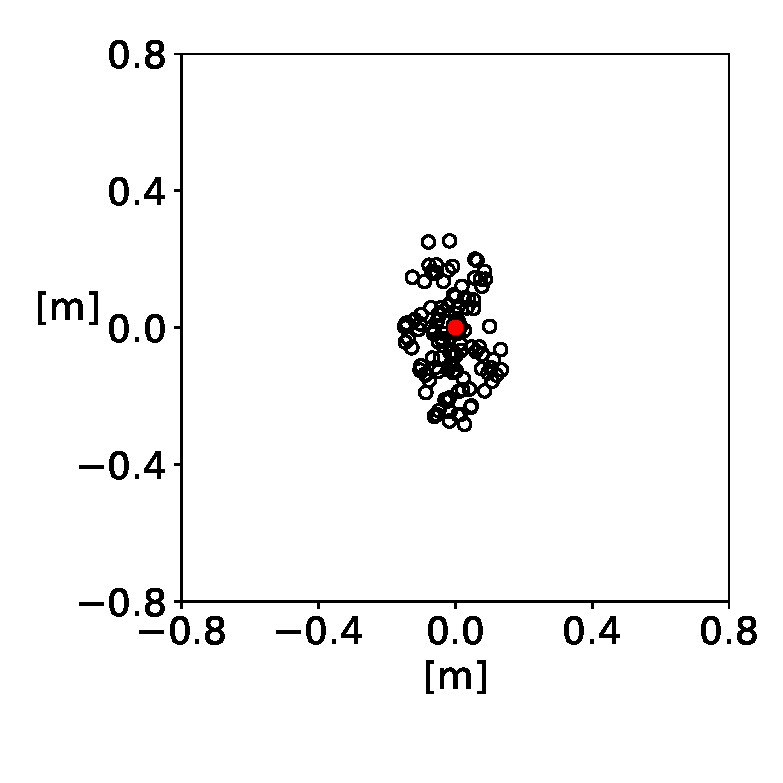
\includegraphics[width=1\hsize]{images/dist1.eps}
                    \caption{基準点1の分布}
                    \label{fig:distribution1}
                \end{minipage}
                \begin{minipage}{0.32\hsize}
                    \centering
                    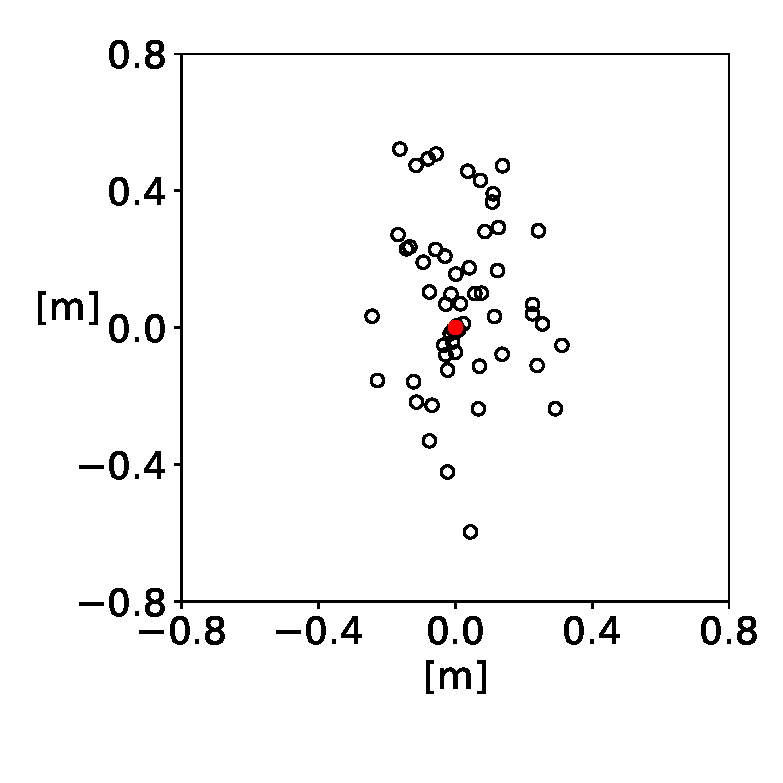
\includegraphics[width=1\hsize]{images/dist2.eps}
                    \caption{基準点2の分布}
                    \label{fig:distribution2}
                \end{minipage}
                \begin{minipage}{0.32\hsize}
                    \centering
                    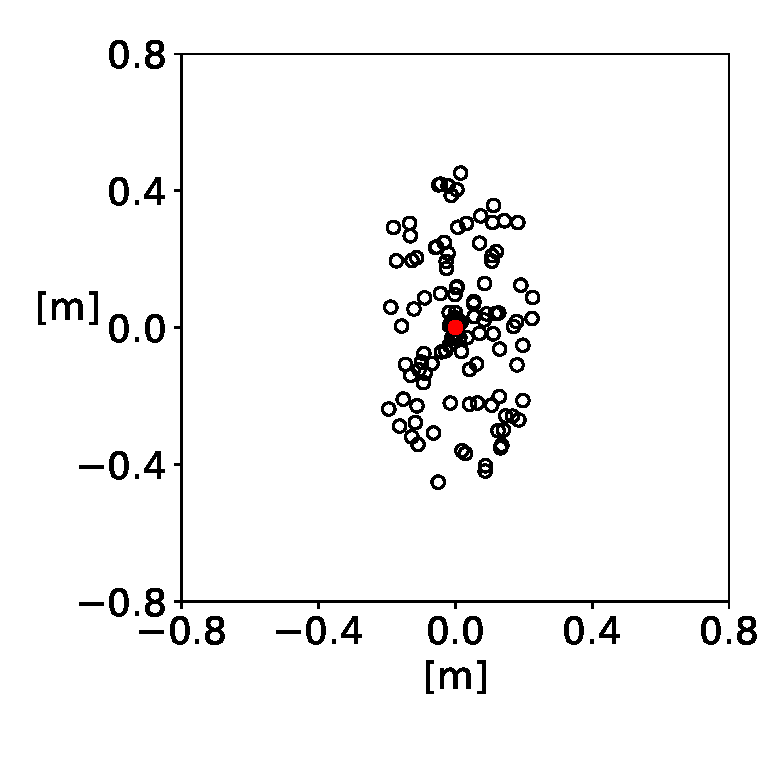
\includegraphics[width=1\hsize]{images/dist3.eps}
                    \caption{基準点3の分布}
                    \label{fig:distribution3}
                \end{minipage}
            \end{figure}

            どの基準点においても、
            縦長の楕円状に分布していることがわかる。
            図\ref{fig:explanation_before}, \ref{fig:explanation_after}に示すように、
            射影変換前の画像においてコートが占める領域に比べ、
            射影変換後の方が縦に長いため、
            縦横に同等に表れたAlphaPoseによる選手の位置の誤差が縦に引き伸ばされた表れたと考えられる。
            この傾向は、3箇所から撮影した全ての映像において同様に確認された。

            \begin{figure}[ht]
                \begin{minipage}{0.49\hsize}
                    \centering
                    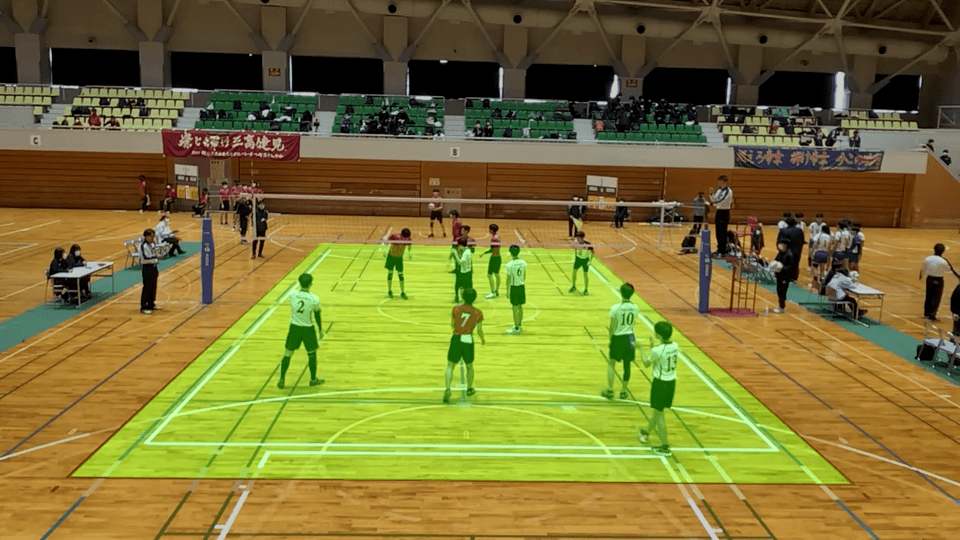
\includegraphics[width=1\hsize]{images/colored_frame.png}
                    \caption{射影変換前の画像においてコートが占める領域}
                    \label{fig:explanation_before}
                \end{minipage}
                \begin{minipage}{0.49\hsize}
                    \centering
                    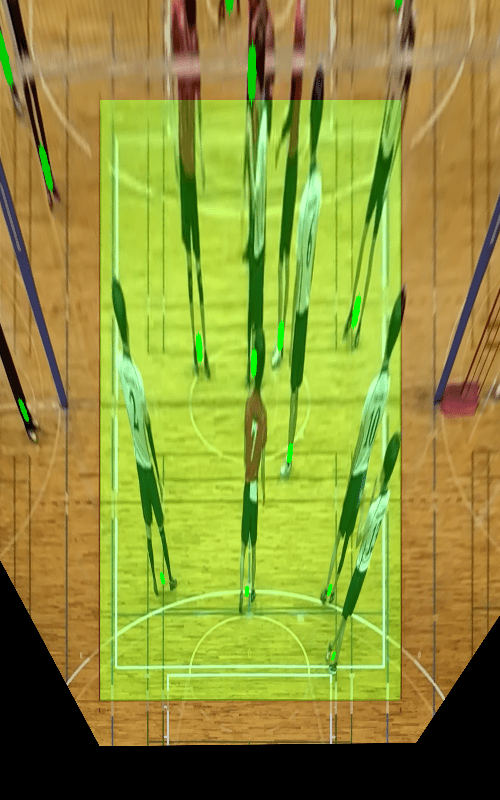
\includegraphics[width=0.7\hsize]{images/colored_warped.png}
                    \caption{射影変換後の画像においてコートが占める領域}
                    \label{fig:explanation_after}
                \end{minipage}
            \end{figure}

\chapter{結論} \label{cha:epilogue}
    \section{まとめ}
        本研究では、情報端末の内蔵カメラを用いて撮影したバレーボールの試合映像と、
        その映像内でコートが写っている位置の情報から、
        自動で選手の位置を推定・追跡した。
        さらに、推定した選手の位置の精度の評価を行った。
        その結果、カメラと選手の距離が増大するほど、
        推定位置の誤差も増大することが予想できた。

    \section{今後の課題} \label{sec:problems}
        本研究では、選手が床上にいる前提で解析を行った。
        しかし、バレーボール選手は試合中にジャンプを行うため、
        空中にいる選手の位置推定も考慮する必要がある。
        また、ボールの位置も同様に空中であるため、
        本研究では推定を行なっていないが、
        Data Volleyのようなプレイの解析を行うためには
        選手の位置だけでなくボールの位置の情報も
        必要となるため、これも同様に検討の必要がある。

    \section{本研究の展望} \label{sec:prospect}
        最後に、本研究の展望を述べる。

        付録\ref{app:3D}に示すVideoPose3D\cite{Dario}は、
        AlphaPoseのようなアルゴリズムを用いて検出した
        選手の2次元姿勢情報から、
        その3次元姿勢を推定するアルゴリズムである。
        これを用いることで、
        映像内の選手の実際の姿勢が推定できる。
        これと本研究で得た選手の位置情報を組み合わせることで、
        バレーボールの試合の3次元再現が可能であると予測する。

        このようなスポーツの試合の3次元再現は、
        Fernandoら\cite{Fernando}がサッカーに注目して行った。
        サッカーのコートは、緑の芝生と白いラインのみで、
        本研究で撮影したバレーボールのコートのように他のスポーツコートのラインが存在しないため、
        多くの先行研究が行われてきた。
        しかし、本研究のようにバレーボールに注目して解析を行った先行研究は少なく、
        先述のようにバレーボールの3次元再現が可能になれば、
        バレーボール指導に大きく役立てられることとなる。

\appendix
\chapter{VideoPose3Dを用いた3次元姿勢推定} \label{app:3D}
    VideoPose3Dを用いて、
    本研究でも用いたAlphaPoseのような姿勢推定アルゴリズムを用いて推定した
    人物の2次元姿勢から、3次元姿勢を推定できる。
    図\ref{fig:videopose2d}, \ref{fig:videopose3d}, \ref{fig:3d}
    にある人物の2次元姿勢、それから推定した3次元姿勢、
    モーションキャプチャを利用して測定した実際の3次元姿勢を示す。

    \begin{figure}[ht]
        \begin{minipage}{0.32\hsize}
            \centering
            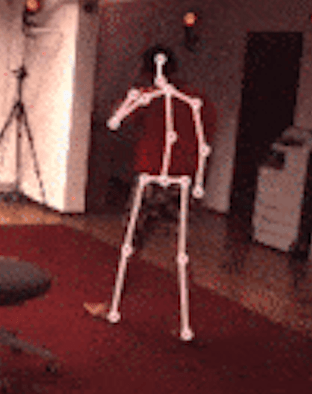
\includegraphics[width=0.7\hsize]{images/videopose2d.png}
            \caption{2次元姿勢}
            \label{fig:videopose2d}
        \end{minipage}
        \begin{minipage}{0.32\hsize}
            \centering
            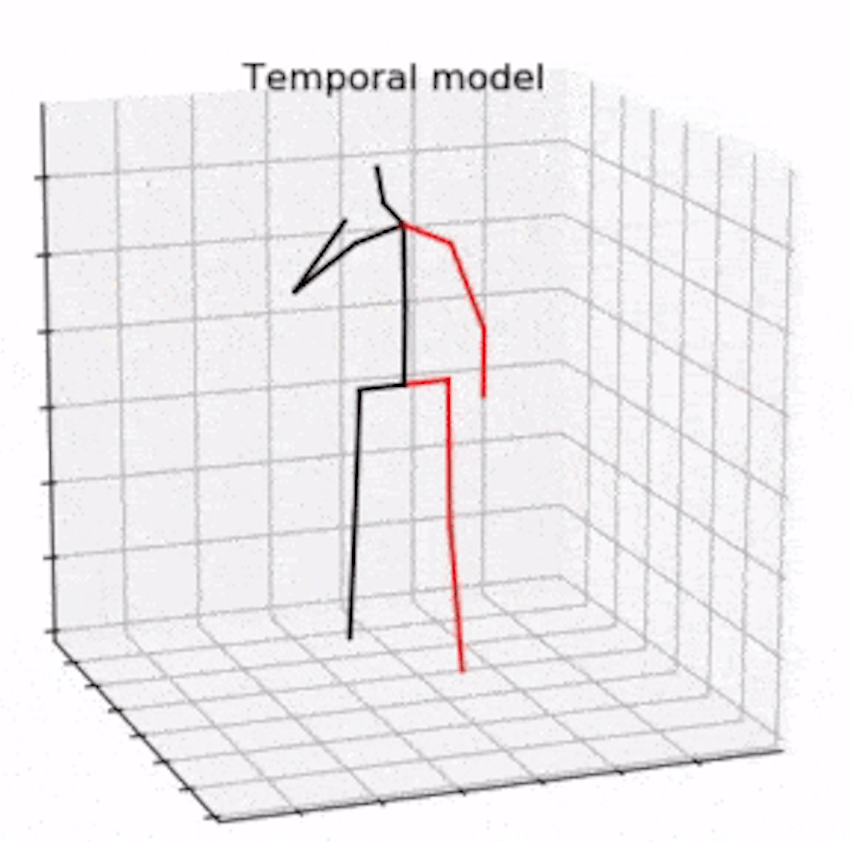
\includegraphics[width=1\hsize]{images/videopose3d.png}
            \caption{推定した3次元姿勢}
            \label{fig:videopose3d}
        \end{minipage}
        \begin{minipage}{0.32\hsize}
            \centering
            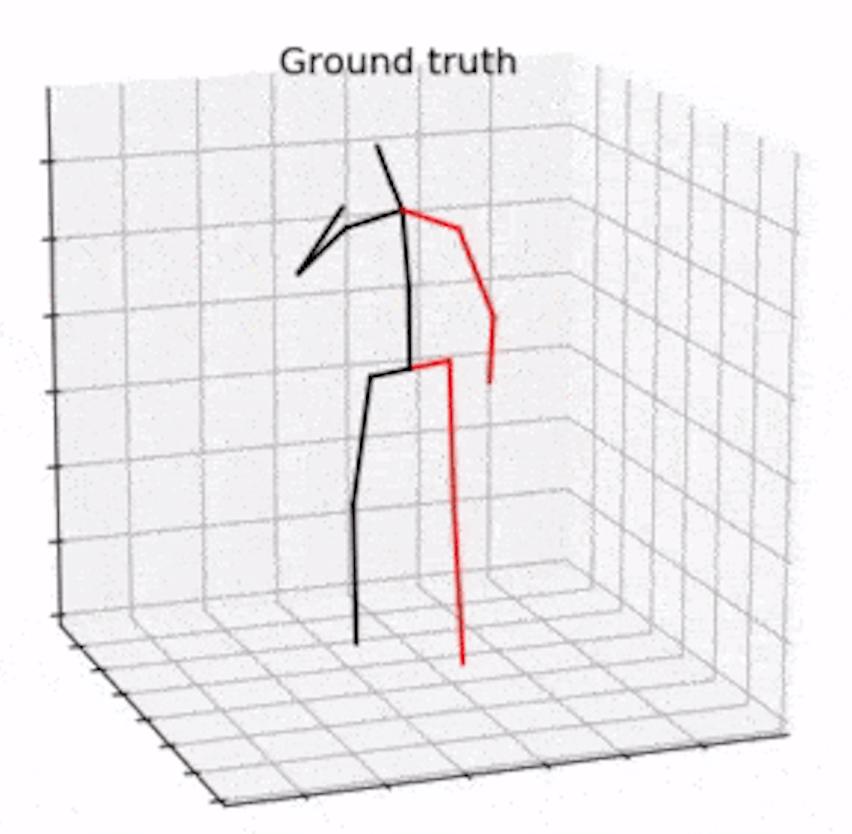
\includegraphics[width=1\hsize]{images/3d.png}
            \caption{実際の3次元姿勢}
            \label{fig:3d}
        \end{minipage}
    \end{figure}

    図\ref{fig:videopose3d}と図\ref{fig:3d}を比較すると、
    人間の目では違いがわからないほどに正確に3次元姿勢が推定できることがわかる。

\chapter{作成したソースコード} \label{app:code}
    以下に、本研究で作成したソースコードを示す。

    リスト\ref{src:html}, \ref{src:css}, \ref{src:js}に示す、
    index.html, index.css, index.jsの3つを合わせて、
    ブラウザ上で動くように作成した。
    これには、\ref{cha:detect}章で述べた、
    コートの四隅を手動で指定するGUIも含まれる。

    また、本研究ではAlphaPoseを用いて映像内の選手の位置を推定した結果を一度ファイルに保存し、
    \ref{src:html}のプログラムで読み込む形をとった。
    AlphaPoseを用いて解析を行う過程は、AlphaPoseの公式ドキュメント
    \footnote{https://github.com/MVIG-SJTU/AlphaPose}を参考にした。

    \begin{lstlisting}[caption=index.html, label=src:html]
<html>
    <head></head>
    <body>
        動画ファイル: <input id="video_input" type="file" accept="video/*"><br>
        解析データ: <input id="pose_input" type="file" accept=".json"><br>
        <div style="position: relative">
            <video id="video" controls></video>
            <canvas id="video_canvas"></canvas>
        </div>
        <canvas id="board_canvas"></canvas>
    </body>
    <link rel="stylesheet" href="index.css">
    <script src="https://docs.opencv.org/3.4.1/opencv.js"></script>
    <script src="index.js"></script>
</html>\end{lstlisting}

    \begin{lstlisting}[caption=index.css, label=src:css]
#video_canvas {
    position: absolute;
    top: 0;
    left: 0;
}

#board_canvas {
    width: 500px;
    height: 800px;
    background: #f3bf88;
    margin-top: 32px;
}\end{lstlisting}

    \begin{lstlisting}[caption=index.js, label=src:js]
const COURT_CANVAS_WIDTH  = 500
const COURT_CANVAS_HEIGHT = 800
const COURT_CORNERS_ON_BOARD = [
    [100, 100],
    [100, 700],
    [400, 700],
    [400, 100]
]
const COURT_GATES_ON_BOARD = [
    [100, 300],
    [400, 300],
    [400, 500],
    [100, 500]
]

const video        = document.getElementById("video")
const videoCanvas  = document.getElementById("video_canvas")
const videoContext = videoCanvas.getContext("2d")
const boardCanvas  = document.getElementById("board_canvas")
const boardContext = boardCanvas.getContext("2d")

const courtCorners = []
const playerPos    = []

var M = null

function getModifiedPos(event) {
    const clientRect = videoCanvas.getBoundingClientRect()

    x = event.pageX - clientRect.left - window.pageXOffset
    y = event.pageY - clientRect.top  - window.pageYOffset

    courtCorners.forEach(function (pos) {
        const [preX, preY] = [...pos]

        if (
            Math.abs(preX - x) / video.videoWidth  < 0.05 &&
            Math.abs(preY - y) / video.videoHeight < 0.05
        ) [x, y] = [preX, preY]
    })

    return [x, y]
}

function draw(pos) {
    videoContext.lineWidth   = 4
    videoContext.strokeStyle = "blue"
    videoContext.fillStyle   = "blue"

    videoContext.clearRect(0, 0, videoCanvas.width, videoCanvas.height)
    videoContext.beginPath()
    videoContext.moveTo(...courtCorners[0])
    for (let i = 1; i < courtCorners.length; i++)
        videoContext.lineTo(...courtCorners[i])
    videoContext.stroke()
    
    courtCorners.forEach(function (corner) {
        videoContext.beginPath()
        videoContext.arc(...corner, 5, 0, 2 * Math.PI, false)
        videoContext.fill()
    })
}

document.getElementById("video_input").addEventListener("change", function () {
    video.src = window.URL.createObjectURL(this.files[0])
    console.log("Loading video...")
})

video.addEventListener("progress", function (event) {
    console.log("Loaded video.")

    videoCanvas.width  = video.videoWidth
    videoCanvas.height = video.videoHeight - 64
    
    console.log("Canvas size changed: " + [videoCanvas.width, videoCanvas.height])
})

video.addEventListener('loadedmetadata', function (e) {
    let time = video.currentTime;
    requestAnimationFrame(function me() {
        if (time !== video.currentTime) {
            time = video.currentTime;
            video.dispatchEvent(new CustomEvent("timeupdate"));
        }
        requestAnimationFrame(me);
    });
});

function warp(point) {
    product = [
        M.data64F[0] * point[0] + M.data64F[1] * point[1] + M.data64F[2],
        M.data64F[3] * point[0] + M.data64F[4] * point[1] + M.data64F[5],
        M.data64F[6] * point[0] + M.data64F[7] * point[1] + M.data64F[8]
    ]

    return [product[0] / product[2], product[1] / product[2]]
}

video.addEventListener("timeupdate", function () {
    const frameRate = 30
    const frame = Math.round(frameRate * video.currentTime)

    draw()
    drawLine()
    videoContext.fillStyle = "green"
    
    for (idx in playerPos[frame]) {
        videoContext.beginPath()
        videoContext.arc(...playerPos[frame][idx], 5, 0, 2 * Math.PI, false)
        videoContext.fill()

        const warpedPlayerPos = warp(playerPos[frame][idx])
        if (warpedPlayerPos[1] > COURT_CANVAS_HEIGHT / 2) {
            boardContext.fillStyle = "blue"
        } else {
            boardContext.fillStyle = "red"
        }

        boardContext.beginPath()
        boardContext.arc(...warpedPlayerPos, 5, 0, 2 * Math.PI, false)
        boardContext.fill()
    }
})

videoCanvas.addEventListener("click", function (event) {
    pos = getModifiedPos(event)

    if (JSON.stringify(courtCorners.slice(-1)[0]) == JSON.stringify(pos)) {
        console.log("Popped court corner: " + courtCorners.pop())
        draw()
    } else {
        courtCorners.push(pos)
        draw()
        console.log("Added court corner: " + pos)

        if (courtCorners.length == 5) {
            M = cv.getPerspectiveTransform(
                cv.matFromArray(4, 1, cv.CV_32FC2, courtCorners.slice(0, 4).flat()),
                cv.matFromArray(4, 1, cv.CV_32FC2, COURT_CORNERS_ON_BOARD.flat())
            )

            console.log("Calculated perspective transform: " + M.data64F)
        }
    }
})

document.getElementById("pose_input").addEventListener("change", function () {
    const reader = new FileReader()
    reader.onload = function () {
        console.log("Loading pose json...")

        let lastImg = ""
        JSON.parse(reader.result).forEach(function (personData) {
            if (lastImg != personData.image_id) {
                playerPos.push({})
                lastImg = personData.image_id
            }

            playerPos.slice(-1)[0][parseInt(personData.idx, 10)] = [
                personData.box[0] + personData.box[2] / 2,
                personData.box[1] + personData.box[3]
            ]
        })
        
        console.log("Loaded pose json.")
    }

    reader.readAsText(this.files[0])
})

function drawLine() {
    boardContext.lineWidth   = 4
    boardContext.strokeStyle = "white"

    boardContext.clearRect(0, 0, boardCanvas.width, boardCanvas.height)
    
    boardContext.beginPath()
    boardContext.moveTo(...COURT_CORNERS_ON_BOARD[0])
    boardContext.lineTo(...COURT_CORNERS_ON_BOARD[1])
    boardContext.lineTo(...COURT_CORNERS_ON_BOARD[2])
    boardContext.lineTo(...COURT_CORNERS_ON_BOARD[3])
    boardContext.closePath()
    boardContext.stroke()

    boardContext.beginPath()
    boardContext.moveTo(...COURT_GATES_ON_BOARD[0])
    boardContext.lineTo(...COURT_GATES_ON_BOARD[1])
    boardContext.lineTo(...COURT_GATES_ON_BOARD[2])
    boardContext.lineTo(...COURT_GATES_ON_BOARD[3])
    boardContext.closePath()
    boardContext.stroke()

    boardContext.beginPath()
    boardContext.moveTo(0, COURT_CANVAS_HEIGHT / 2)
    boardContext.lineTo(COURT_CANVAS_WIDTH, COURT_CANVAS_HEIGHT / 2)
    boardContext.stroke()
}

drawLine()\end{lstlisting}

\begin{thebibliography}{99}
    \bibitem{JSA}{
        日本スポーツ協会、``公認スポーツ指導者養成テキスト 共通科目III''、2016
    }
    \bibitem{Watanabe}{
        渡辺裕、``スポーツ情報処理の研究開発動向''、映像情報メディア年報2018シリーズ、2018
    }
    \bibitem{Nakai}{
        中井聖 他、 ``バレーボールコート内の既知点を用いた3次元座標空間の再構築方法の精度とその特徴''、
        日本バレーボール学会、2017
    }
    \bibitem{Kitahara}{
        北原格、太田友一、 ``多視点映像の融合によるスポーツシーンの自由視点映像生成 : 3次元形状表現用平面の適応的配置''、
        電子情報通信学会技術研究報告 \textit{(PRMU)} パターン認識・メディア理解、2001
    }
    \bibitem{Joseph}{
        Joseph R., et al.,
        ``You Only Look Once: Unified, Real-Time Object Detection'',
        In \textit{Computer Vision and Pattern Recognition (CVPR) 2015}, 2015
    }
    \bibitem{Microsoft}{
        Tsung-Yi L., et al.,
        ``Microsoft COCO: Common Objects in Context'',
        In \textit{Computer Vision and Pattern Recognition (CVPR) 2014}, 2014
    }
    \bibitem{Zhe}{
        Zhe C., et al.,
        ``OpenPose: Realtime Multi-Person 2D Pose Estimation using Part Affinity Fields'',
        In \textit{Computer Vision and Pattern Recognition (CVPR) 2018}, 2018
    }
    \bibitem{Hao}{
        Hao-Shu F., et al.,
        ``RMPE: Regional Multi-person Pose Estimation'',
        In \textit{Computer Vision and Pattern Recognition (CVPR) 2016}, 2016
    }
    \bibitem{kashika}{
        可視化情報学入門編集委員会、
        ``可視化情報学入門''、
        東京電機大学出版局、1994
    }
    \bibitem{Dario}{
        Dario P., et al.,
        ``3D human pose estimation in video with temporal convolutions and semi-supervised training'',
        In \textit{Computer Vision and Pattern Recognition (CVPR) 2019}, 2019
    }
    \bibitem{Fernando}{
        Fernando D., et al.,
        ``Soccer Field Lines Determination and 3D Reconstruction'',
        In \textit{International Conference on Geometry and Graphics (ICGG) 2020}, 2020
    }
\end{thebibliography}
\end{document}